\documentclass{standalone}
    \begin{document}
    
        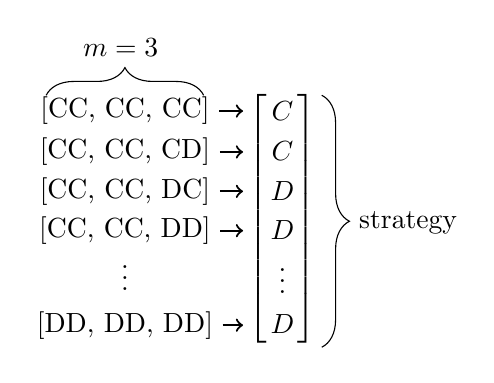
\begin{tikzpicture}[draw, minimum width=1cm, minimum height=0.5cm]

    
        \tikzstyle{state}=[minimum width=0.5cm, font=\boldmath];
    
        \node  (1) at (0,0) [state] {[CC, CC, CC]};
        \node  (2) at (0,-.52) [state] {[CC, CC, CD]};
        \node  (3) at (0,-1.02) [state] {[CC, CC, DC]};
        \node  (4) at (0,-1.52) [state] {[CC, CC, DD]};
        \node  (5) at (0,-2.02) [state] {$\vdots$};
        \node  (6) at (0,-2.72) [state] {[DD, DD, DD]};
        \node (7) at (2, -1.37) {
            $\arraycolsep=1.2pt\def\arraystretch{1.2}\left[\begin{array}{c}
                C  \\
                C  \\
                D  \\
                D  \\
                $\vdots$ \\
                D  \\
            \end{array}\right]$
            };

        \draw (1) edge[out=0, in=180, ->, thick] node [left] {} (1.5, 0);
        \draw (2) edge[out=0, in=180, ->, thick] node [left] {} (1.5, -.52);
        \draw (3) edge[out=0, in=180, ->, thick] node [left] {} (1.5, -1.02);
        \draw (4) edge[out=0, in=180, ->, thick] node [left] {} (1.5, -1.52);
        \draw (6) edge[out=0, in=180, ->, thick] node [left] {} (1.5, -2.72);

        \draw [decorate,decoration={brace,amplitude=10pt}] (-1, .2) -- (1, .2) node [above, xshift=-30pt, yshift=10pt] {$m=3$};
        \draw [decorate,decoration={brace,amplitude=10pt}] (2.5, .2) -- (2.5, -3) node [right, xshift=10pt, yshift=45pt] {strategy};

        \end{tikzpicture}
    
    \end{document}